% Example LaTeX document for GP111 - note % sign indicates a comment
\documentclass[12pt]{article}
% Default margins are too wide all the way around. I reset them here
\usepackage{amsmath}
%\usepackage{mathtools}
\usepackage{graphicx}
\usepackage[danish]{babel}
\usepackage{listings}
\usepackage{color}
\usepackage[utf8]{inputenc}
\usepackage{hyperref}
\usepackage{float}

\definecolor{codegreen}{rgb}{0,0.6,0}
\definecolor{codegray}{rgb}{0.5,0.5,0.5}
\definecolor{codepurple}{rgb}{0.58,0,0.82}
\definecolor{backcolour}{rgb}{0.95,0.95,0.92}
 
\lstdefinestyle{mystyle}{
    backgroundcolor=\color{backcolour},   
    commentstyle=\color{codegreen},
    keywordstyle=\color{magenta},
    numberstyle=\tiny\color{codegray},
    stringstyle=\color{codepurple},
    basicstyle=\footnotesize,
    breakatwhitespace=false,         
    breaklines=true,                 
    captionpos=t,                    
    keepspaces=true,                 
    numbers=left,                    
    numbersep=5pt,                  
    showspaces=false,                
    showstringspaces=false,
    showtabs=false,                  
    tabsize=2
}
 
\lstset{style=mystyle}
\renewcommand\lstlistingname{Fil}
\renewcommand{\abstractname}{Hej}
\addto{\captionsdanish}{\renewcommand{\abstractname}{Abstract}}
\numberwithin{equation}{section}

\pagestyle{headings}

\begin{document}
\title{Numerisk Integration}
\author{Søren Fritzbøger 3F\\
HTX Hillerød - Erhversskolen Nordsjælland\\
Vejleder: Stig og CHR}
\renewcommand{\today}{2. Februar 2015}
\maketitle

\begin{abstract}
This article demonstrates a basic set of LaTeX formatting commands.
Compare the typeset output side-by-side with the input document.smøøre
\end{abstract}

\tableofcontents

\section{Forklaring af numerisk integration}



\section{Trapezmetoden}
\label{sec:trapezmetoden}
Trapezmetoden er en af flere metoder til at finde areal under en funktion. Det er en af de mere præcise metoder, da den, i modsætning til højre-, venstre- og middelsum, laver en trapez og ikke en firkant.
\subsection{Bevis for trapezmetoden}
Ved at bruge trapezmetoden kan vi tilnærmelsesvist finde det bestemte integral, selv for funktioner, hvor man ikke direkte kan bestemme det bestemte integral. Et eksempel på dette er funktionen $f(x)=e^{-x^{2}}$.
For at bestemme arealet under en funktion vil vi gerne nærme os det bestemte integral.
\begin{equation}
\int_{a}^{b}f(x)dx \nonumber
\end{equation}
Når $a<b$ og $f$ er kontinuerlig og differentiabel i intervallet $[a;b]$, kan vi bruge trapezmetoden til at udregne det tilnærmelsesvist bestemte integral, som er arealet under funktionen.\\
Som navnet trapezmetoden så fint hentyder til, opdeler vi vores funktion i en trapez, som vi udregner arealet af. Dette er illustreret på figur \ref{fig:trapezmetoden}
\begin{figure}[H]
\centering
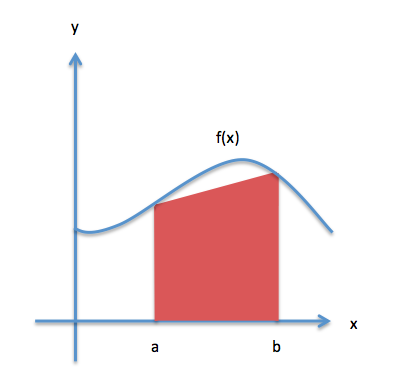
\includegraphics[scale=0.5]{Billeder/trapezmetoden.png}
\caption{Trapezmetoden}
\label{fig:trapezmetoden}
\end{figure}


På figur \ref{fig:trapezmetoden} kan man se, hvordan trapezmetoden opdeler en parabel i en trapez. Denne trapez har intervallet $[a;b]$. Længden $a=f(a)$ og længden $b=f(b)$. Formlen for arealet af en trapez ses i formel \eqref{eq:trapezareal}
\begin{equation}
\label{eq:trapezareal}
A=\frac{1}{2}h\cdot(a+b)
\end{equation}
\begin{figure}[H]
	\centering
	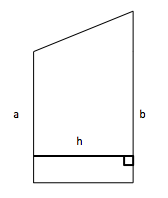
\includegraphics[scale=0.8]{Billeder/Trapez}
	\caption{Trapez}
	\label{fig:trapez}
\end{figure}

Som man kan se på figur \ref{fig:trapez}, er $a$ og $b$ er sidelænger og $h$ er højden. I et trapez er højden defineret som afstanden mellem de to parallelle linjestykker, i dette tilfælde $a$ og $b$, som man kan se illustreret på figur \ref{fig:trapez}
\\\\
Som man kan se på figur \ref{fig:trapez} svarer højden $h$ til afstanden mellem $a$ og $b$, som svarer til $h=b-a$. Når man indsætter henholdsvis $a$ og $b$ værdien ind i vores $f(x)$ funktion, får vi vores $y$ værdi, som svarer til længden af henholdsvis $a$ og $b$.
Hvis vi indsætter dette i arealet for en trapez, får vi derfor:
\begin{align}
A &= \frac{1}{2}h\cdot(a+b) &\Rightarrow \nonumber
\\ &= \frac{1}{2}(b-a) \cdot (a+b) &\Rightarrow \nonumber
\\ &= \frac{b-a}{2} (a+b) &\Rightarrow \nonumber
\intertext{i stedet for $a$ og $b$ indsættes højderne på trapezens sider, $f(a)$ og $f(b)$} \nonumber
\\ &= \frac{b-a}{2} (f(a)+f(b))
\\ \intertext{Arealet af denne trapez svarer tilnærmelsesvist til arealet under funktionen. Så derfor kan vi sige at arealet af trapezen tilnærmelsesvist svarer til værdien af det bestemte integral:} \nonumber
\\ \int_{a}^{b}f(x) &\approx \frac{b-a}{2} (f(a)+f(b))
\end{align}

\subsubsection{Opdeling i intervaller}
\label{sec:opdelingtrapezmetoden}
Som man kan se på figur \ref{fig:trapezmetoden} er trapezmetoden meget upræcis i forhold til det bestemte integral. Dette kan man forbedre ved at dele intervallet $[a;b]$ op i flere delintervaller, $n$. Dvs. at vi deler vores funktion op i mindre intervaller, som vi så finder arealet af med trapezmetoden. Disse delintervaller kalder vi for $x_0, x_1, \cdots x_n$. Vi skal bruge højden på trapezen, som er længden af delintervallet $x_0 - x_1$. I dette tilfælde svarer det til:
\begin{align}
h = x_1-x_0 = x_2-x_1 = \cdots = x_n - x_{n-1}
\end{align}
Ud fra dette kan vi bestemme at højden, $h$, må svare til intervallet $[a;b]$ opdelt i $n$ intervaller:
\begin{align}
h=\frac{b-a}{n}
\end{align}
Det samlede areal under funktionen kan betegnes som summen af alle delintervallerne:
\begin{align}
A &= \lim\limits_{n \rightarrow \infty} \sum_{i=1}^{n} \frac{h}{2}(f(x_{i}) + f(x_{i+1}))
\approx \int_{a}^{b}f(x) &\text{hvor }h=\frac{b-a}{n}
\end{align}
Når n går mod uendelig bliver vores delinterval infinitesimalt lille, hvilket vil sige at summen af alle trapezarealerne nærmer sig det bestemte integral. Det bestemte integral svarer faktisk til at vi deler arealet op i uendelige små og uendelig mange led.
\\\\
For at udlede dette til formlen for trapezmetoden bliver vi nødt til at opskrive dette på en lidt anden måde.
\begin{align}
A &= \frac{h}{2}(f(x_0)+ f(x_1)) + \frac{h}{2}(f(x_1)+ f(x_2)) + \cdots + \frac{h}{2}(f(x_{n-1})+ f(x_n)) \nonumber
\\ &= h(\frac{1}{2}f(x_0) + \frac{1}{2}f(x_1)) + h(\frac{1}{2}f(x_1) + \frac{1}{2}f(x_2)) + \cdots + h(\frac{1}{2}f(x_{n-1}) + \frac{1}{2}f(x_n)) \nonumber
\\ &= h \cdot \frac{1}{2}f(x_0) + h \cdot \frac{1}{2}f(x_1) + h \cdot \frac{1}{2}f(x_1) + h \cdot \frac{1}{2}f(x_2) + \cdots + h \cdot \frac{1}{2}f(x_{n-1}) + h \cdot \frac{1}{2}f(x_n) \nonumber
\end{align}
Dette bliver reduceret til formlen for trapezmetoden \eqref{eq:trapezmetoden}
\begin{align}
\label{eq:trapezmetoden}
\boxed{\int_{a}^{b}f(x) \approx \frac{h}{2}(f(x_0) + 2f(x_1) + \cdots + 2f(x_{n-1}) + f(x_n))} \\ \text{Hvor } h=\frac{b-a}{n} \nonumber
\end{align}

\section{Simpsons metode}
En anden metode til tilnærmelsesvist at udregne arealet under en funktion er simpsons-metoden, som virker ved at dele funktionen op i mindre parabler, man så finder arealet under. Denne metode er mere præcis end trapezmetoden\footnote{\cite[side 15]{2012matA}}, og giver derfor et resultat som oftest har en meget lille afvigelse fra det korrekte resultat, det bestemte integral.
\subsection{Bevis for Simpsons metode}
Simpsons metode er som nævnt, en anden metode til tilnærmelsesvist at finde det bestemte integral, selv for funktioner, hvor man ikke direkte kan bestemme det bestemte integral. Med trapezmetoden, se afsnit \ref{sec:trapezmetoden}, brugte man en ret linje fra $f(a)$ til $f(b)$ i intervallet $[a;b]$, hvilket selvfølgelig ikke er helt præcis, da en funktion ikke nødvendigvis er ret. Med Simpsons metode opdeler man intervallet $[a;b]$ i en parabel ud fra 3 punkter, $a,b,c$. Disse tre punkter kan bruges til at opstille en simplere parabel, som vi så kan regne arealet under. Parablens ligning ser således ud: $y=ax^2+bx+c$

\subsubsection{Opdeling i intervaller}

\clearpage
\addcontentsline{toc}{section}{Litteratur}
\begin{thebibliography}{9}

\bibitem{JohnsonUtah}
  	Christopher R. Johnson,
  	\emph{Denne kilde er et dokument med beviser, beskrivelse og andet af numerisk integration.}.\\
  	Hamlet Project, 
  	Department of Computer Science,
	University of Utah,
	\url{http://www.cs.utah.edu/~zachary/computing/lessons/uces-13/uces-13/contents-node1.html}
	
\bibitem{html5canvas}
	@mattmight,
	\emph{En ``tutorial'' der viser hvordan man tegner en graf vha. html5 og canvas}.\\
	http://matt.might.net/articles/rendering-mathematical-functions-in-javascript-with-canvas-html/

\bibitem{au}
	Aalborg Universitet,
	\emph{Et foredag fra Aalborg Universitet omhandlende Numerisk Integration}.\\
	http://staff.iha.dk/jse/bioproces/Forelaesningsnoter/BI1MAT1/\\Numeriske\%20metoder\%201.pdf
\bibitem{2012matA}
	Undervisningsministeriet,
	\emph{Forberedelse til Matematik A højere teknisk eksamen 2012},
	\url{http://uvm.dk/~/media/UVM/Filer/Udd/Gym/PDF12/Proever\%20og\%20eksamen/120608\%20Mat\%20A\%20htx\%20Forberedelsesmateriale.pdf}

\end{thebibliography}

\end{document}